
%(BEGIN_QUESTION)
% Copyright 2006, Tony R. Kuphaldt, released under the Creative Commons Attribution License (v 1.0)
% This means you may do almost anything with this work of mine, so long as you give me proper credit

A very useful principle in physics is the {\it Ideal Gas Law}, so called because it relates pressure, volume, molecular quantity, and temperature of an ideal gas together in one neat mathematical expression:

$$PV = nRT$$

\noindent
Where,

$P$ = Absolute pressure (atmospheres)

$V$ = Volume (liters)

$n$ = Gas quantity (moles)

$R$ = Universal gas constant (0.0821 L $\cdot$ atm / mol $\cdot$ K)

$T$ = Absolute temperature (K)

\vskip 10pt

Although this ``law'' is not perfectly accurate for real gases, especially at high pressures and/or near the point of liquefaction, it is quite accurate for air near ambient temperature and pressure.

One very practical application of this law is found in a method for generating low air pressures such as those easily measured by water- or oil-based manometers.  Most mechanical air compressors generate pressures far exceeding the range of all but the largest manometers.  Though it is possible to purchase precision pressure regulators for reducing such large pressures down to a level measurable by a manometer, these devices are expensive.  An alternative is to generate the air pressure with a hand pump (such as a bicycle tire pump) connected to a relatively large pressure vessel:

$$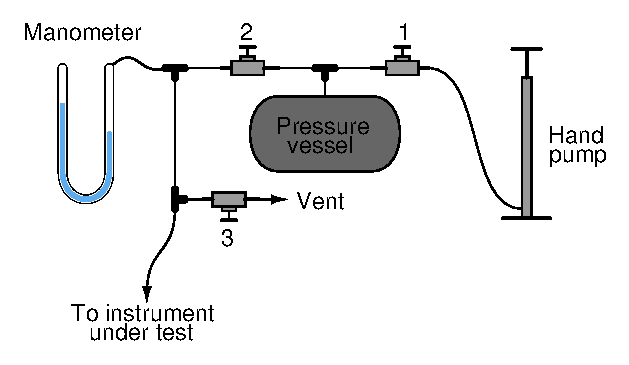
\includegraphics[width=15.5cm]{i00286x01.eps}$$

Without the volume of the pressure vessel connected to the tubing system, the air pressure would increase dramatically for each stroke of the air pump.  With the pressure vessel connected, each pump stroke contributes a much smaller amount of additional pressure to the system.  Use the Ideal Gas Law equation to explain why this is.

\underbar{file i00286}
%(END_QUESTION)





%(BEGIN_ANSWER)

Actuating the hand pump introduces more air molecules to the system ($n$).  Assuming temperature ($T$) remains constant, the air pressure ($P$) will increase in inverse proportion to the volume ($V$) of the pressure vessel for each additional stroke of the pump.

\vskip 10pt

Follow-up question: If we wished the pressure to increase {\it less} for every stroke of the pump, would we want a smaller pressure vessel or a larger pressure vessel?  Explain your answer.

\vskip 10pt

Challenge question: suppose a technician follows these steps in using this system.

\begin{itemize}
\item{} Close valve 2, open valves 1 and 3
\item{} Pump several strokes' worth of air into the pressure vessel
\item{} Close valves 1 and 3
\item{} {\it Slowly} open valve 2 until manometer registers desired pressure, then close
\end{itemize}

Is the air pressure going to the instrument under test greater than, less than, or equal to the air pressure in the vessel?

%(END_ANSWER)





%(BEGIN_NOTES)

Stated using calculus (differential) notation, the pressure vessel's volume relates to the rate of pressure change with respect to air quantity as such:

$${dP \over dn} = {RT \over V}$$

Given that $R$ is a constant and $T$ is generally constant as well (in addition to being difficult to precisely manipulate), we may simplify the expression as such:

$${dP \over dn} \propto {1 \over V}$$

If students experience confusion over this principle, ask them the following question: which will take longer; pumping up a bicycle tire with a bicycle pump, or pumping up a truck tire with the same bicycle pump?  Anyone who has ever had to pump up a car or truck tire with nothing more than a bicycle pump knows how long it takes!  This is nothing more than an application of the Ideal Gas Law.

%INDEX% Calibration, generating low air pressures using a bicycle (hand) pump
%INDEX% Physics, static fluids: ideal gas Law

%(END_NOTES)


